\section{Generating X-rays}

\begin{figure}
	\centering
	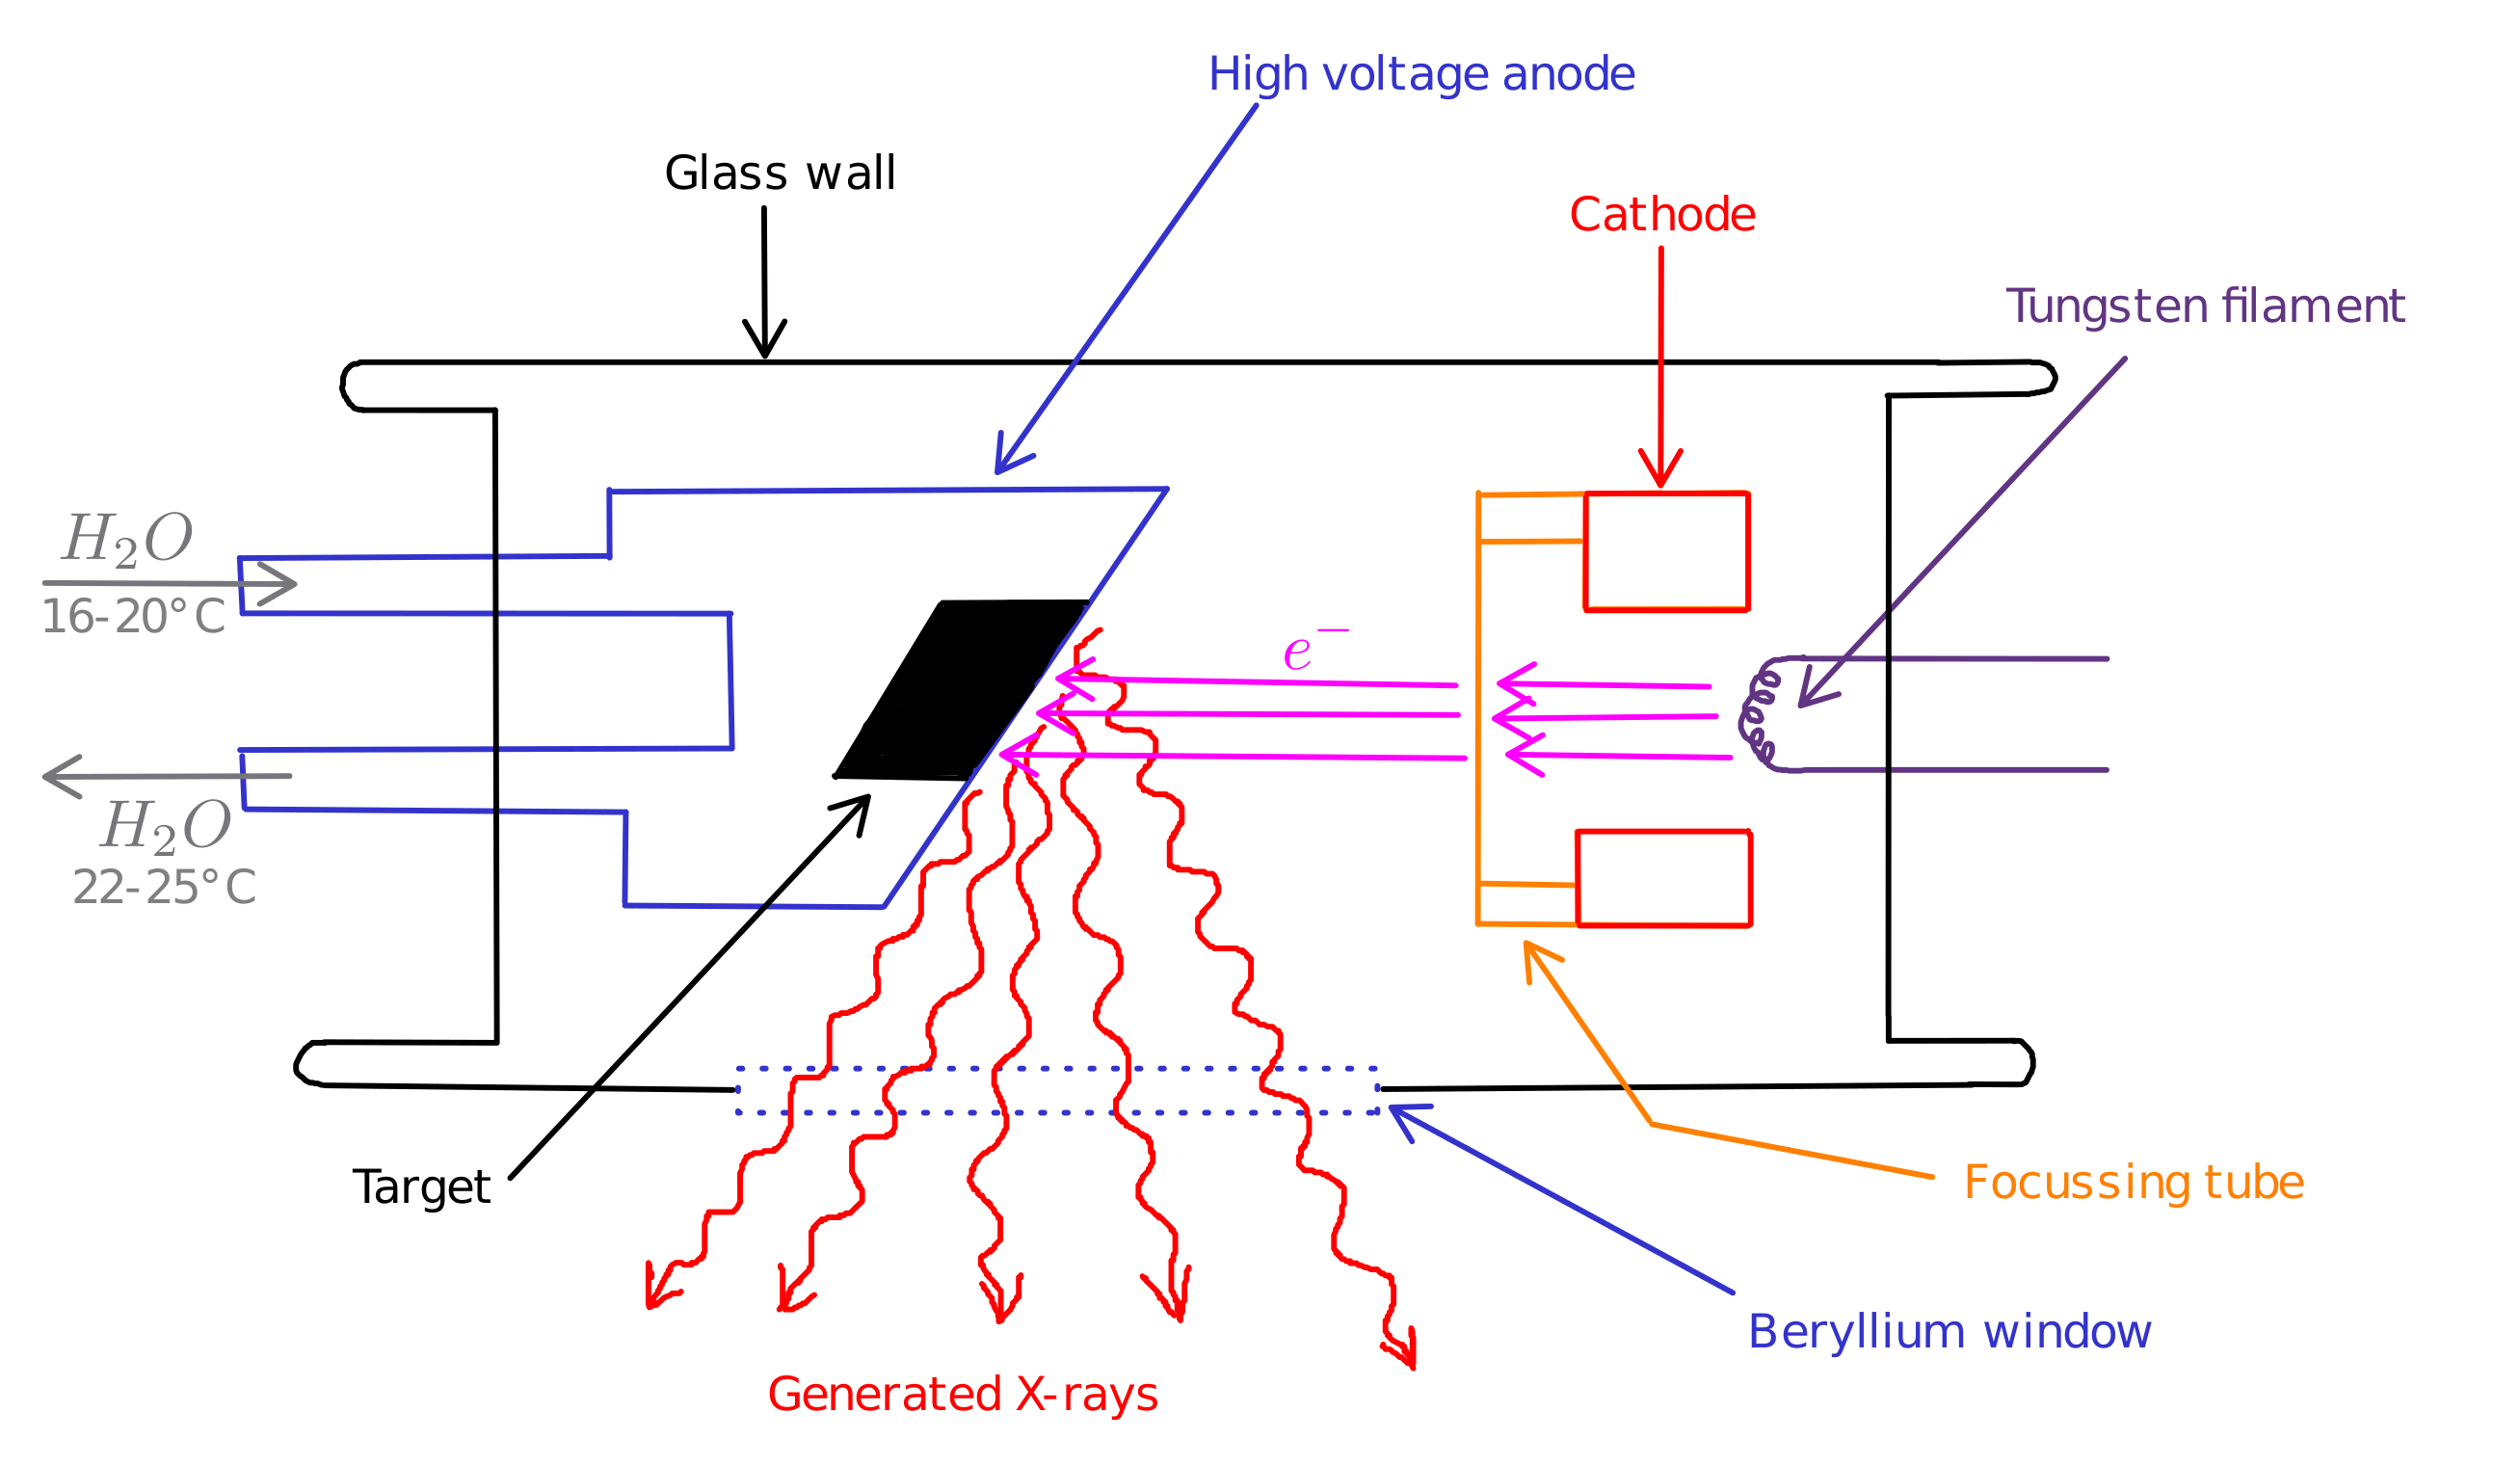
\includegraphics[scale=0.14]{xray_tube.png}
	\caption{\label{fig:xray_tube}Schematic of a X-ray tube.}
\end{figure}

	Figure~\ref{fig:xray_tube} shows the schematic of a X-ray tube. The potential difference between the anode to cathode is around $20-60~\si{kV},$ while the Tungsten filament is supplied a current of $\sim 2-50~\si{mA}.$ The target is composed of the material from which we want to generate the X-rays (generally Cu, Mo or Ag). The Beryllium window provides a transparent region for the generated X-rays to pass through.
	
	The tube is not allowed to cool down between experiments. In the stand-by state, the filament current is reduced to around $\SI{5}{mA}$ and the anode potential is also reduced to $\SI{20}{kV}.$ When data collection is started, the anode voltage is increased to $>\SI{50}{kV}$ and the current in the Tungsten filament is increased to $\SI{40}{mA}.$ In this state, the heated Tungsten filament generates electrons, which are then accelerated and finally hit the target at the anode.

\begin{figure}[h]
	\centering
	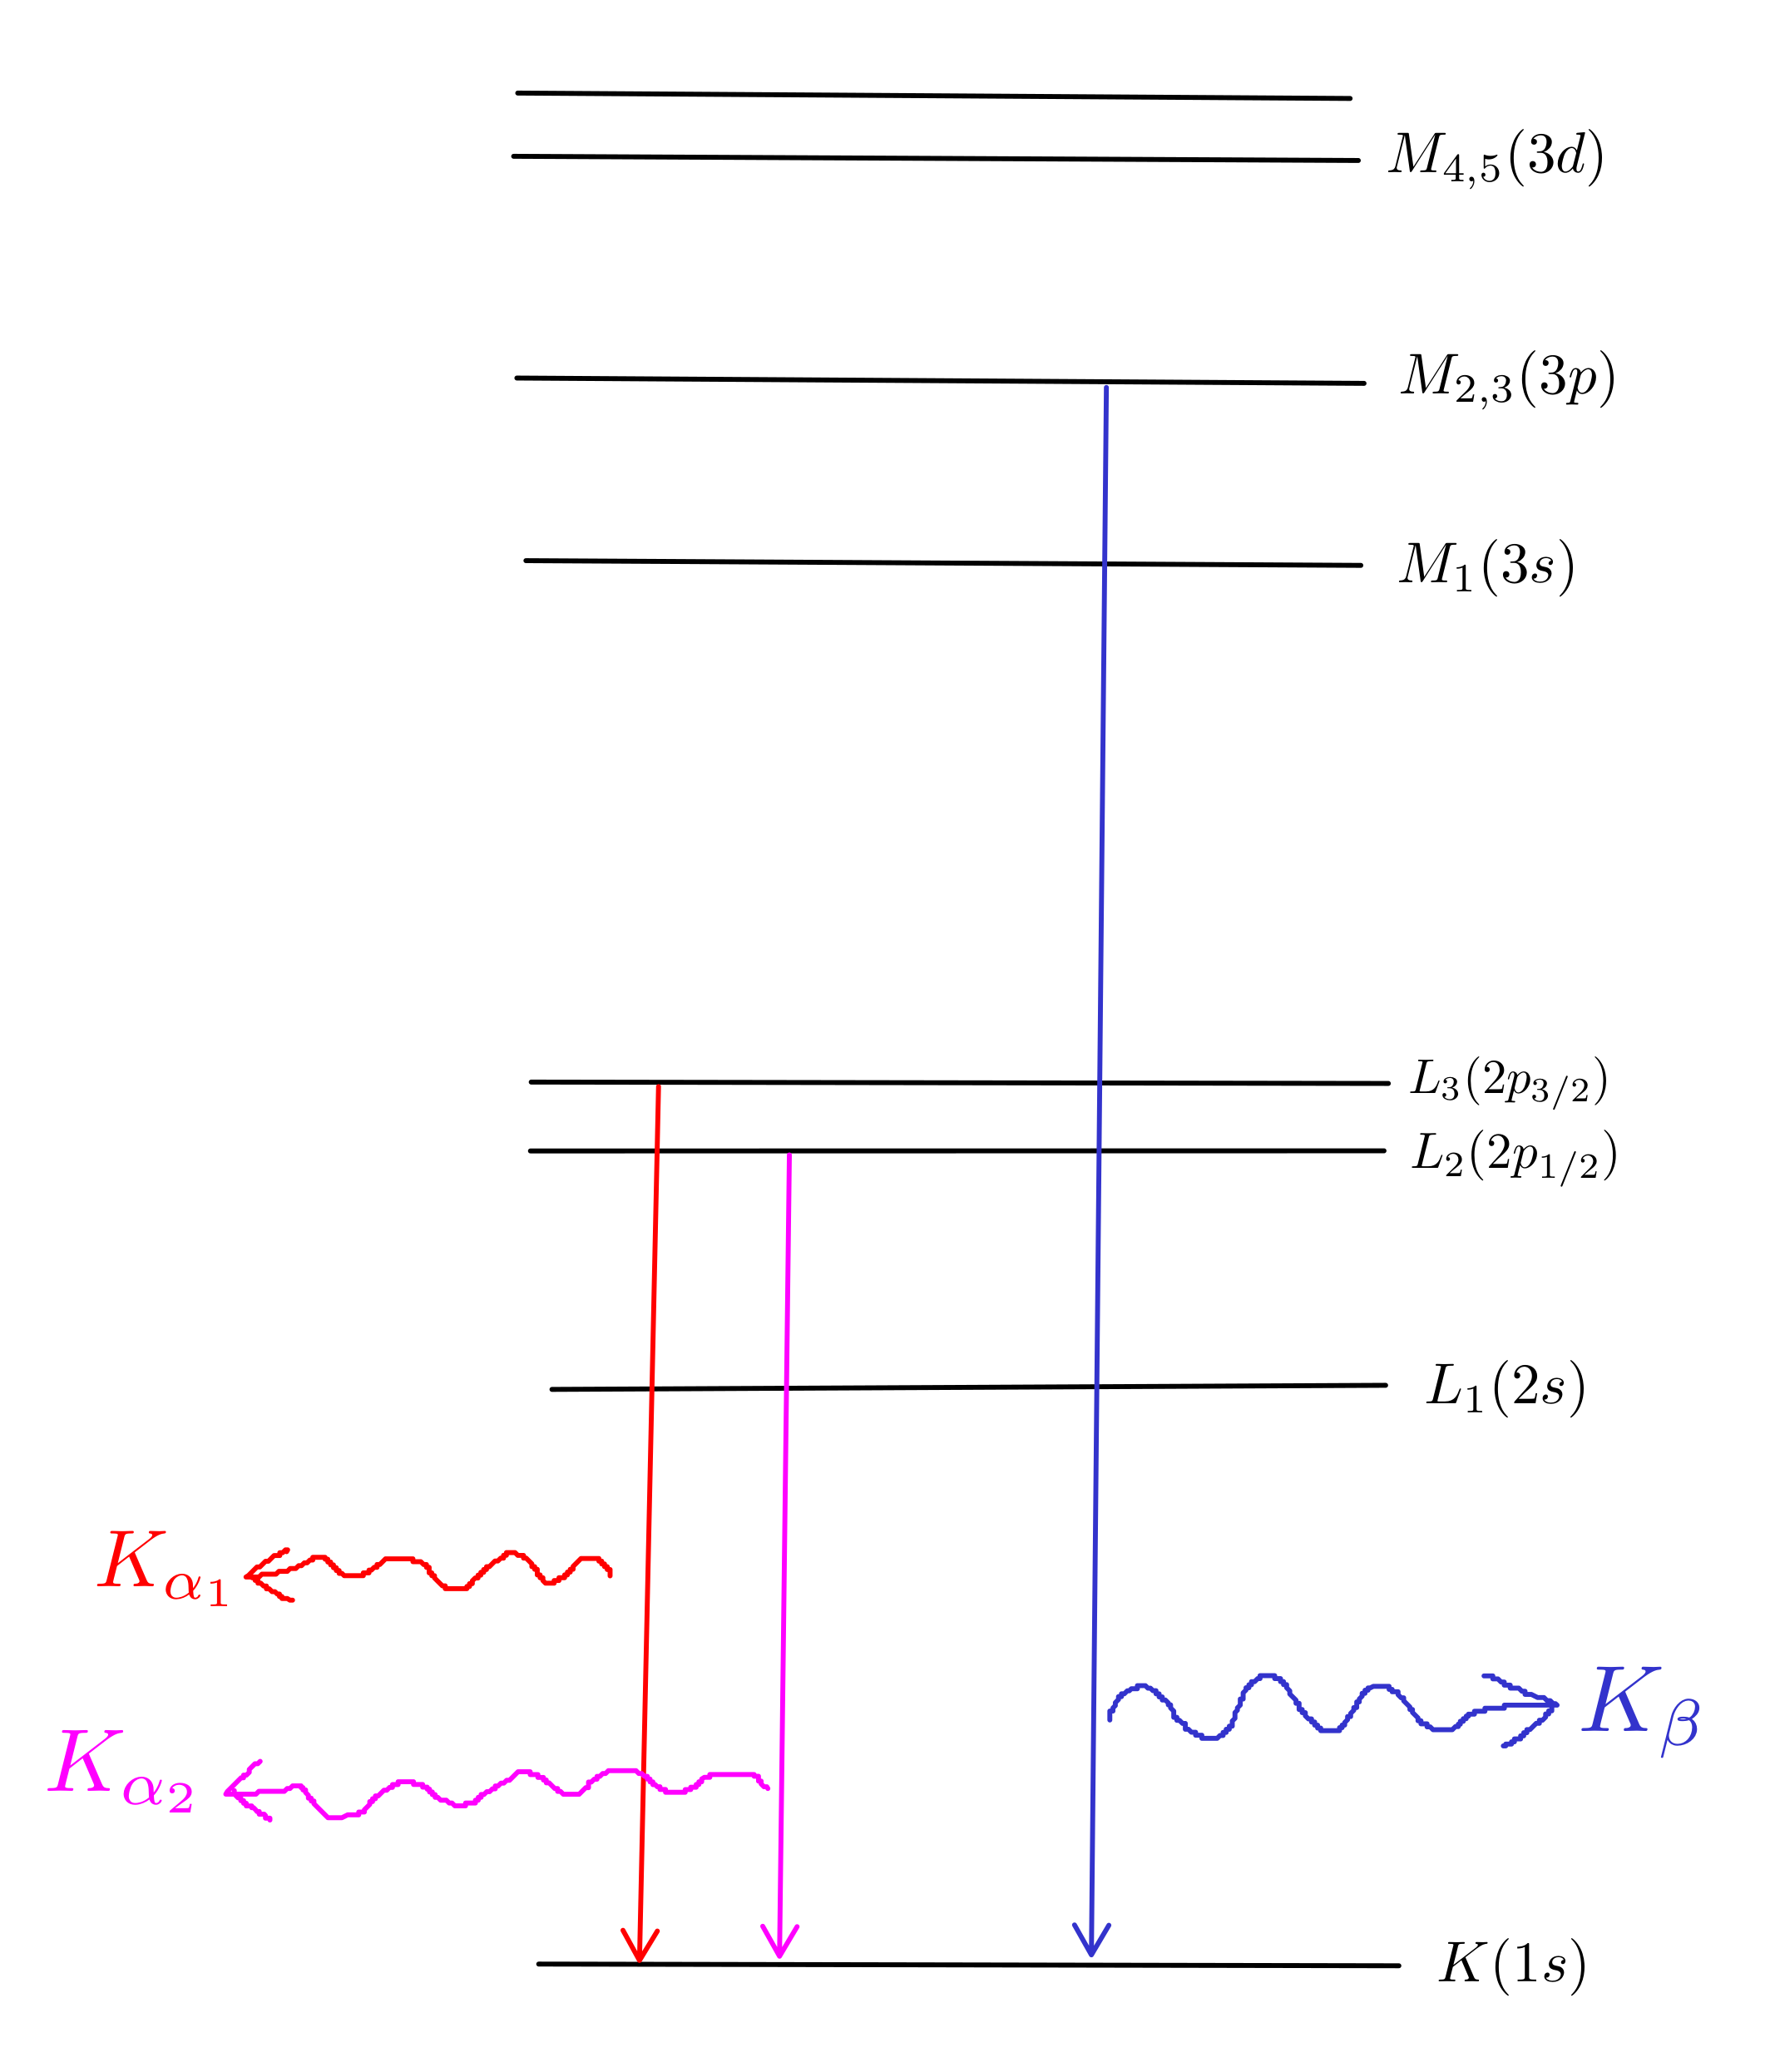
\includegraphics[scale=0.1]{characteristic_xray_transitions.png}
	\caption{\label{fig:xray_transitions}Transitions giving rise to characteristic X-rays.}
\end{figure}
	
	These electrons are able to knock out electrons from the K-shell of an atom in the target. Once an electron is removed from the K-shell, electrons from higher energy levels release energy and come to the K-shell. This release energy is the characteristic X-rays of the material. There are three possible transitions which give rise to X-rays of three different wavelengths. These are shown in figure~\ref{fig:xray_transitions}.
	
\begin{figure}[h]
	\centering
	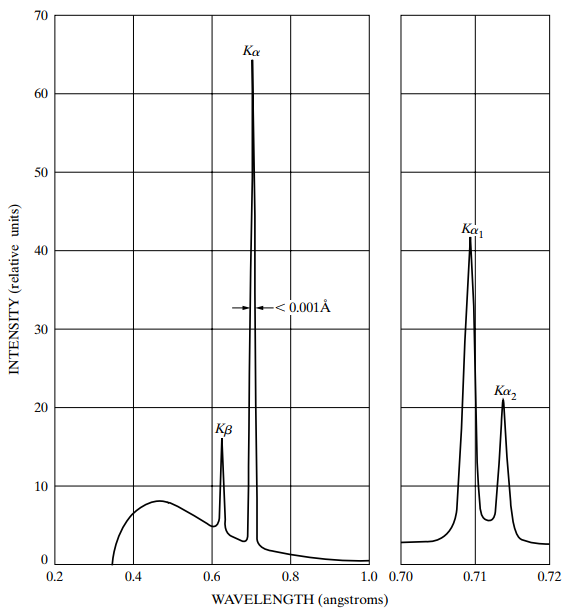
\includegraphics[scale=0.6]{xray_peaks.png}
	\caption{\label{fig:xray_spctra_Cu_Mo}X-ray spectra of $\mathrm{Mo}$ at $\SI{35}{kV}$. The $K_\alpha$ is shown expanded on the right. Picture courtesy:~\cite{Cullity2014}.}
\end{figure}
	
	The X-ray spectra of Mo is shown in figure~\ref{fig:xray_spctra_Cu_Mo}. The $K_\alpha$ peaks are very close to each other. The wavelengths can be found in table~\ref{tab:wavelengths}. The background radiation or white X-rays is attributed to Bremstrahlung, which is the radiation emitted by electrons when they are decelerated in the X-ray tube.
	
\begin{table}
	\centering
	\caption{\label{tab:wavelengths}Wavelengths of characteristic radiations of Cu and Mo.}
	\begin{tabular}{|c|C|C|C|C|C|c|}
	
		\hline
		
		Source & K_{\alpha_1} (\si{\angstrom}) & K_{\alpha_2} (\si{\angstrom}) & \multicolumn{1}{c|}{\makecell{$K_\alpha$ (average)\\($\si{\angstrom}$)}} & K_\beta (\si{\angstrom}) & Z & $\beta$ filter\\
		
		\hhline{|=|=|=|=|=|=|=|}
		
		Cu & 1.5405 & 1.5433 & 1.5418 & 1.3922 & 29 & Ni (Z = 28) \\
		
		\hline
		
		Mo & 0.7093 & 0.7136 & 0.7107 & 0.6393 & 42 & Nb (Z = 41)\\
		
		\hline
	
	\end{tabular}
\end{table}
	
	We use monochromatic radiation for X-ray diffraction experiments. For this, we have to filter out the unwanted $K_\beta$ and $K_{\alpha2}$ radiations. To filter the $K_\beta$ spectra, we use a $\beta$-filter. The  $\beta$-filters used for Cu and Mo are listed in table~\ref{tab:wavelengths}.
	
	To separate $K_{\alpha1}$ from $K_{\alpha2}$, we use a crystal monochromator. For this, a $\mathrm{Ge}$ crystal is cut along the $(111)$ plane, and the beam with mixed radiation is shined on this plane. Since the two radiations have different wavelengths, they will diffract at two different angles. We can eliminate the unwanted $K_{\alpha2}$ in this way. However, note that \ifnt{the intensity of the reflected beam will fall severely} due to loss of intensity upon reflection.